\documentclass[submission]{grattan}\usepackage[]{graphicx}\usepackage[]{color}
%% maxwidth is the original width if it is less than linewidth
%% otherwise use linewidth (to make sure the graphics do not exceed the margin)
\makeatletter
\def\maxwidth{ %
  \ifdim\Gin@nat@width>\linewidth
    \linewidth
  \else
    \Gin@nat@width
  \fi
}
\makeatother

\definecolor{fgcolor}{rgb}{0.345, 0.345, 0.345}
\newcommand{\hlnum}[1]{\textcolor[rgb]{0.686,0.059,0.569}{#1}}%
\newcommand{\hlstr}[1]{\textcolor[rgb]{0.192,0.494,0.8}{#1}}%
\newcommand{\hlcom}[1]{\textcolor[rgb]{0.678,0.584,0.686}{\textit{#1}}}%
\newcommand{\hlopt}[1]{\textcolor[rgb]{0,0,0}{#1}}%
\newcommand{\hlstd}[1]{\textcolor[rgb]{0.345,0.345,0.345}{#1}}%
\newcommand{\hlkwa}[1]{\textcolor[rgb]{0.161,0.373,0.58}{\textbf{#1}}}%
\newcommand{\hlkwb}[1]{\textcolor[rgb]{0.69,0.353,0.396}{#1}}%
\newcommand{\hlkwc}[1]{\textcolor[rgb]{0.333,0.667,0.333}{#1}}%
\newcommand{\hlkwd}[1]{\textcolor[rgb]{0.737,0.353,0.396}{\textbf{#1}}}%
\let\hlipl\hlkwb

\usepackage{framed}
\makeatletter
\newenvironment{kframe}{%
 \def\at@end@of@kframe{}%
 \ifinner\ifhmode%
  \def\at@end@of@kframe{\end{minipage}}%
  \begin{minipage}{\columnwidth}%
 \fi\fi%
 \def\FrameCommand##1{\hskip\@totalleftmargin \hskip-\fboxsep
 \colorbox{shadecolor}{##1}\hskip-\fboxsep
     % There is no \\@totalrightmargin, so:
     \hskip-\linewidth \hskip-\@totalleftmargin \hskip\columnwidth}%
 \MakeFramed {\advance\hsize-\width
   \@totalleftmargin\z@ \linewidth\hsize
   \@setminipage}}%
 {\par\unskip\endMakeFramed%
 \at@end@of@kframe}
\makeatother

\definecolor{shadecolor}{rgb}{.97, .97, .97}
\definecolor{messagecolor}{rgb}{0, 0, 0}
\definecolor{warningcolor}{rgb}{1, 0, 1}
\definecolor{errorcolor}{rgb}{1, 0, 0}
\newenvironment{knitrout}{}{} % an empty environment to be redefined in TeX

\usepackage{alltt}
\usepackage{dblfloatfix}
\usepackage{longtable}

% add_to_dictionary: taxfilers lamington LITO bn perc
% may_be_left_unreferenced: tbl:2

\addbibresource{bib/put-new-refs-here.bib}

\date{May 2018}
\title{Submission to the Senate Economics Legislation Committee inquiry into the Treasury Laws Amendment (Personal Income Tax Plan) Bill 2018}
\author{Danielle Wood, John Daley, and Hugh Parsonage}











\IfFileExists{upquote.sty}{\usepackage{upquote}}{}
\begin{document}


\begin{summary}

We welcome the opportunity to comment on the Treasury Laws Amendment (Personal Income Tax Plan) Bill 2018.

The tax cuts proposed by the Personal Income Tax Plan are the largest ever proposed in a Federal Budget. The third tranche of the Tax Plan will ultimately comprise almost half the annual cost of the Tax Plan.

This substantial reduction in revenue is not obviously consistent with the Federal Government's medium-term fiscal strategy of budget surpluses on average over the economic cycle. On current projections these will be achieved only if Australia experiences a lengthy period of unprecedented economic calm and fiscal restraint.

While fairness is in the eye of the beholder, the Tax Plan should be evaluated relative to the progressivity of the income tax system today. While the level of progressivity is a value choice, changes to such a fundamental issue should be made consciously, in the light of comprehensive analysis of proposed changes.

Without tax cuts, the income tax system will become less progressive. Bracket creep has the biggest effect on the average tax rates of taxfilers in the middle of the distribution (who earn around \$44,000 a year). 

The Tax Plan does not unwind the reduction in progressivity as a result of bracket creep. The Tax Plan reduces average tax rates by about 1 percentage point for most taxpayers. But it reduces average tax rates by substantially more for the top 20 per cent of taxpayers -- except for the top 1 per cent of income earners.

As a result, by 2027-28, about 3 per cent of the tax burden will be shifted from the top 20 per cent of income earners to those lower down.

The outcomes vary a little depending on wages growth. If wages grow more slowly than projected, then the combination of bracket creep and the Tax Plan will be a little less regressive than if wages grow as projected in the budget.

Other analysis is less relevant to fairness. The proportion of the tax cuts over eleven years going to high-income earners distracts from the \emph{ongoing} impact of the tax cuts after that period. The proportion of taxfilers in the top or second-top tax bracket, or the proportion of tax paid by them, is likewise a distraction because it does not indicate whether the overall system is becoming more or less progressive.
\end{summary}




\chapter{How large are the tax cuts?}\label{chap:how-large-are-the-tax-cuts}

The tax cuts proposed by the Treasury Laws Amendment (Personal Income Tax Plan) Bill 2018 are the largest ever proposed in a Federal Budget. We calculate that once all phases of the Tax Plan are in force, they will reduce income tax collected by \$18~billion in 2024-25.%
  \footnote{The analysis in this submission updates and refines quantitative analysis Grattan Institute has previously published, including \textcite{DaleyWood2018}.}
The largest previous changes we have identified were the tax cuts announced in May 2006, projected to cut income tax by \$10 billion in 2009-10.\footcite[][23]{Treasury2006}

The Government has not made available estimates of the annual impact of the tax cuts beyond the forward estimates period. With-holding this information cannot be justified on the basis that it is unreliable%
  \footcite{Murphy2018}
given that the Government has been prepared to provide information on the total impact of each component of the package over a ten-year period, which can only be calculated by adding the impact of each year.

Grattan Institute has estimated the impact of the tax cuts using the 2015-16 2\% individuals sample file, assuming the Budget's estimates of wage growth, and using the Budget's estimates of labour force growth.

On these assumptions, as shown in  \Vref{fig:1},\footnote{Our calculations roughly correspond to published Treasury projections of the cumulative impact of the package components. The major variance is that Treasury projections assume less impact in the first year of each change, because they take into account that a portion of collections will be taxed at the rates applicable in the previous year.}
the first tranche of the tax cuts, which introduces a Low and Middle Income Tax Offset (which we have labelled the ``Lamington'' for convenience), will reduce tax collections by \$4.6~billion in 2021-22. The second tranche, will reduce tax collections by a further \$5.7~billion in 2022-23. The third tranche, will reduce tax collections by a further \$7.7~billion in 2024-25. This third tranche, will ultimately comprise almost half the annual cost of the Personal Income Tax Plan.

\begin{figure}
\caption{Tax cuts will reduce tax collections by \$22 b in 2024-25}\label{fig:1}
\units{Annual impact of Personal Income Tax Plan, \$ billion (nominal)}
\begin{knitrout}
\definecolor{shadecolor}{rgb}{0.969, 0.969, 0.969}\color{fgcolor}
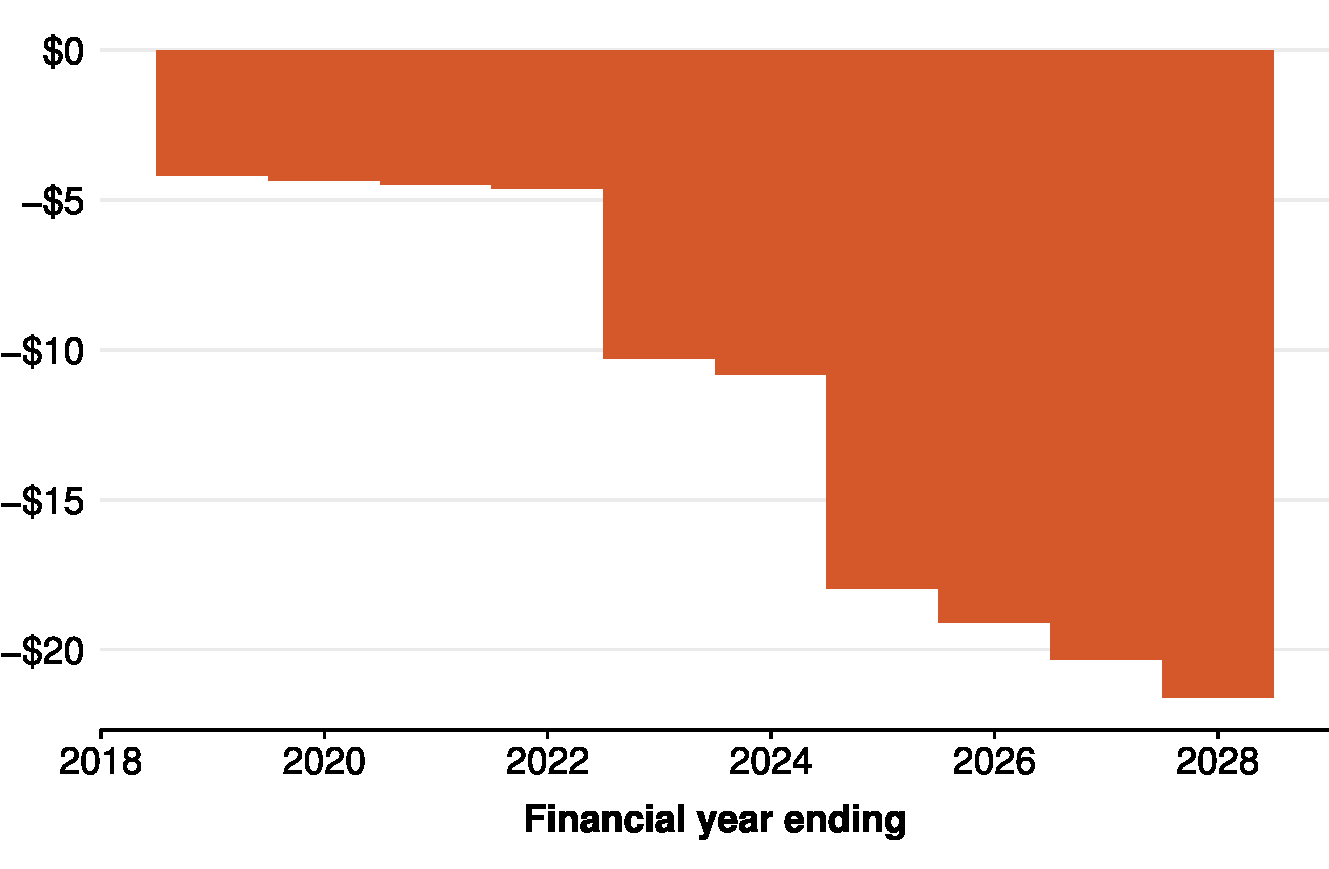
\includegraphics[width=4.47222in,height=2.92631723826715in]{atlas/fig1-1} 

\end{knitrout}
%% \includegraphics[width=4.47847in,height=3.35885in]{media/image2.emf}


\noteswithsource{Assumes wages and population growth as per 2018-19 Budget.}%
{\textcite{ATO2018}; Grattan analysis}
\end{figure}

\chapter{Are the tax cuts affordable? }\label{chap:are-the-tax-cuts-affordable}

The Personal Income Tax Plan commits the Federal Budget to a very substantial reduction in revenue.

The Personal Income Tax Plan is not obviously consistent with the Government's medium-term fiscal strategy ``to achieve budget surpluses, on average, over the course of the economic cycle.''\footcite[][3--7]{Treasury2018a}
The Commonwealth has posted substantial budget deficits since 2009-10 of around 3 per cent of GDP\@.
The 2018-19 Budget effectively delays reaching a surplus of 1 per cent of GDP from 2022-23 to 2026-27.\footcite[][3--15]{Treasury2018a}
The budget will only be in surplus if one assumes an economic cycle of almost 30 years, which is historically unlikely.

The slow consolidation of the Commonwealth's budget position is shown by the slow reduction in the Commonwealth net debt position from 18 per cent of GDP today to 4 per cent of GDP in 2028-29. Of course, this depends in part on the projected value of the Commonwealth's assets: gross debt is only projected to fall from \$561 billion in 2018-19 to \$532 billion by 2028-29.\footcite[][3--16]{Treasury2018a}

In short, the Personal Income Tax Plan is consistent with the Government's medium-term fiscal strategy only if Australia experiences a long period of unprecedented economic calm and fiscal restraint.

The fiscal problems of committing to large tax cuts in the future were illustrated in the late 2000s. The Government announced and legislated tax cuts in 2007 of \$5 billion a year, with an additional \$3 billion a year to take effect in 2008-09.\footcite[][3]{Treasury2007}
By the time these took effect, the Global Financial Crisis had pushed the Federal Budget into a substantial deficit. But politically it was too hard to unwind tax cuts that had already been legislated.

The 2018 tax cuts are even further into the future: half of the proposed reduction -- \$11~billion a year -- only comes into force in six years time. Based on history, a material economic downturn at some time in the interim is a significant possibility.


\chapter{Are the tax cuts fair?}\label{chap:are-the-tax-cuts-fair}

Fairness is in the eye of the beholder. But much of the debate about the Personal Income Tax Plan has been muddied by misleading statistics and comparisons. While we do not have a view on whether the tax cuts are ``fair'', we believe that the public is entitled to a debate, informed by evidence, that clarifies the issues.

First, this debate needs a baseline for measuring whether the tax cuts make the system more or less ``fair''. We believe the most useful baseline is the progressivity of the tax system -- do relatively high-income earners bear more or less of the tax burden?

Second, the debate needs an assessment against this baseline.

And third, the debate needs to understand how the results might vary if the economy turns out differently from projections.

On each of these issues, the debate does \emph{not} need contributions that are unclear about their baseline, or that use statistics which appear to measure progressivity, but do not in fact do so.

\section{Baseline}\label{sec:baseline}

The core fairness question for the income tax system is its level of progressivity. In other words, \textbf{what proportion of income tax is paid} by those with relatively high incomes? Progressivity remains constant if a tax cut reduces tax paid by the same proportion for all taxpayers. Progressivity remains roughly (but not precisely) the same if \textbf{average tax rates change by the same amount} across the income distribution.

There are alternatives. A number of these imply that every tax change should make the system \emph{more} progressive. Taken to extremes, these would ultimately lead to a tax system in which a very small number of people paid all of the income tax collected.

One could look for a constant \textbf{dollar value of tax cuts} across the income distribution. This is the effect of the ``Lamington'' component of the Personal Income Tax Plan. If this were the only form of tax cuts, it would lead to a much more progressive income tax because those with higher incomes currently pay more tax in absolute terms.

One could compare the \textbf{proportion of the budget cost of tax cuts} across the income distribution.
But because higher-income earners pay a higher proportion of total tax (they earn more, and they get taxed at a higher rate), a tax cut that has no impact on progressivity will necessarily provide larger tax cuts to those on higher incomes.

One could compare the \textbf{percentage increase in post-tax income} across the income distribution.\footcite[][11]{Phillips2018}
While this sounds more like a proportionate outcome, it implies an increasingly progressive tax system. By definition, post-tax income is a lower proportion of pre-tax income for those on higher incomes. For example, if there were a uniform 2 per cent increase in post-tax income, a middle-income earner would pay 11 per cent less tax while a high-income earner would pay 5 per cent less tax.\footnote{Assumes a middle-income earner with income of \$50,000 and an average tax rate of 15\%, and a higher (approximately 90\textsuperscript{th} percentile) income earner with income of \$120,000 and an average tax rate of 29\%.}

Other alternatives might appear to be proxies for judging that a tax change is progressive, but can conceal actual changes in either direction.

The \textbf{percentage of tax paid by people on a particular tax bracket} provides no insight into progressivity.\footnote{For example, the Budget Overview highlights how an increasing proportion of taxpayers will be on the top marginal tax rate: \textcite[][9]{Treasury2018b}. See also \textcite[][7--8]{Treasury2018c}.}
For example, with no changes to tax rates, as wages grow, the top bracket will include a greater \emph{proportion of taxpayers}, and so the proportion of tax paid by them will also grow. Nevertheless, the top 10 per cent of taxpayers would pay a \emph{lower} proportion of income tax.



The \textbf{percentage of tax savings under the Tax Plan over eleven years} provides no insight into progressivity. Some have argued that the Tax Plan is fair because the third stage is only a minority of the total revenue foregone over the next eleven years.\footnote{For example, \textcite{Kelly2018}.}
But while the components of the Tax Plan will be \emph{introduced} in a staggered way, their \emph{impact} will be permanent and ongoing. So although the last tranche comprises only 29 per cent of the cost of the package over eleven years,\footcite[][2]{Treasury2018c}
it will cost approximately 40~per~cent in each year thereafter.\footnote{Based on Grattan analysis: see \Vref{fig:1} above.}

Consequently, none of the alternatives illuminate a discussion about fairness. A simple analysis of what proportion of income tax is paid by each decile is preferable.

Of course, the optimal progressivity of a tax system is a fundamental value choice between more equal outcomes on the one hand, and less government intervention into the rewards that markets deliver on the other. If the tax cuts aim to shift the balance towards a more or less progressive tax system, that is a legitimate choice, but it should be made explicitly.

This baseline also assumes that taxable income is a reasonable measure of total income. But in fact, taxable income excludes some capital gains,\footcite{DaleyWood2016-Negative-Gearing-CGT} and earnings from superannuation,%
  \footcites{DaleyCoatesWood-2015-Super-tax-targeting}{Daley-etal-2016-Assessing-2016-super-tax-reforms} which disproportionately benefit those with more taxable income. While these exclusions should be carefully scrutinised, that scrutiny is best undertaken by reviewing these policies directly rather than adjusting general rates of income tax.

The progressivity of the tax system can be judged by looking at a proportion of all adults, all those who file a tax return, or all households.\footcite{Gothe}
Depending on the population chosen, the ``top 20 per cent'' pays a different share of income tax.

In our view, it is better to analyse all taxfilers rather than all adults.\footnote{Analysis by Deloitte Access Economics looks at the percentage of tax paid by the top 20 per cent of adults: \textcite{Greber}.}
Most adults who do not file a tax return are retirees with little income other than the pension. These retirees are unlikely to pay income tax under any scenario. We think it is appropriate to exclude them from the analysis because the key issue in understanding the progressivity of the tax system is the distribution of the tax burden between those people who might plausibly pay income tax.

Alternatively, the population of households can be analysed. This takes it account how a person's resources in practice depend on the total income of their household and the number of people in it.
  \footcite{Phillips2018}
It also allows analysis to take into account welfare that depends on the household's income, such as Family Tax Benefit. However, data sources for households are less reliable and less detailed than the data available for individual taxpayers.

\section{Bracket creep impact}\label{sec:bracket-creep-impact}



\begin{table}
\caption{Bracket creep will make the tax system less progressive; the Tax Plan does little to unwind this}\label{tbl:1}
% latex table generated in R 3.5.0 by xtable 1.8-2 package
% Sun Jun 03 21:44:48 2018
\begin{tabularx}{\columnwidth}{rRRRR}
  \toprule
  \multicolumn{5}{c}{\textbf{Share of income tax}}\\
 \cmidrule(lr){1-5}
 \textbf{Percentile} & \textbf{Share of income} & \textbf{2017-18} & \textbf{2027-28 baseline} & \textbf{2027-28 budget}\\
 \midrule
1-10 & 0.4\% & 0\% & 0\% & 0\% \\ 
  11-20 & 2.2\% & 0\% & 0\% & 0\% \\ 
  21-30 & 3.6\% & 0.4\% & 0.8\% & 0.7\% \\ 
  31-40 & 5.0\% & 1.6\% & 2.2\% & 2.1\% \\ 
  41-50 & 6.5\% & 3.4\% & 4.2\% & 4.2\% \\ 
  51-60 & 8.0\% & 5.8\% & 6.2\% & 6.3\% \\ 
  61-70 & 9.8\% & 8.5\% & 8.6\% & 8.9\% \\ 
  71-80 & 12.2\% & 12.1\% & 12.1\% & 12.3\% \\ 
  81-90 & 15.7\% & 17.8\% & 17.8\% & 17.7\% \\ 
  91-99 & 26.5\% & 32.9\% & 32.3\% & 31.5\% \\ 
  Top 1\% & 9.9\% & 17.5\% & 15.8\% & 16.3\% \\ 
   \bottomrule
\end{tabularx}

\end{table}

At present, the top 20 per cent of income earners -- who earn 51~per~cent of taxable income -- pay 68~per~cent of income tax. As shown in \Vref{tbl:1}, without changes to income tax rates, bracket creep will make the system \emph{less} progressive, and they will only pay 66~per~cent of income tax.



Although many think of ``bracket creep'' as a problem for high income earners, it most affects those in the middle of the income distribution (around \$45,000 taxable income per year). They are affected not because they move into a higher tax bracket, but because increases in income as a result of inflation are taxed at their \emph{marginal} tax rate, which is typically much higher than their \emph{average} tax rate. Overall, bracket creep affects people more if the percentage point difference between their average and marginal tax rate is large, and if their total income is relatively small.


\section{Progressivity of the tax cuts}\label{sec:progressivity-of-the-tax-cuts}

Taken as a whole, the Tax Plan will not unwind bracket creep's gradual reduction of the progressivity of the tax system. Even with the Tax Plan, average tax rates are forecast to be higher for all taxpayers in 2027-28 -- except for very high-income earners who aren't much affected by bracket creep in the first place, as shown in \Vref{fig:bracket-creep-hurts-middle-incomes-most}.

\begin{figure}
\caption{Bracket creep hurts middle incomes most; the Tax Plan doesn't unwind this}\label{fig:bracket-creep-hurts-middle-incomes-most}
\units{Average tax rates by taxable income percentile}
\begin{knitrout}
\definecolor{shadecolor}{rgb}{0.969, 0.969, 0.969}\color{fgcolor}
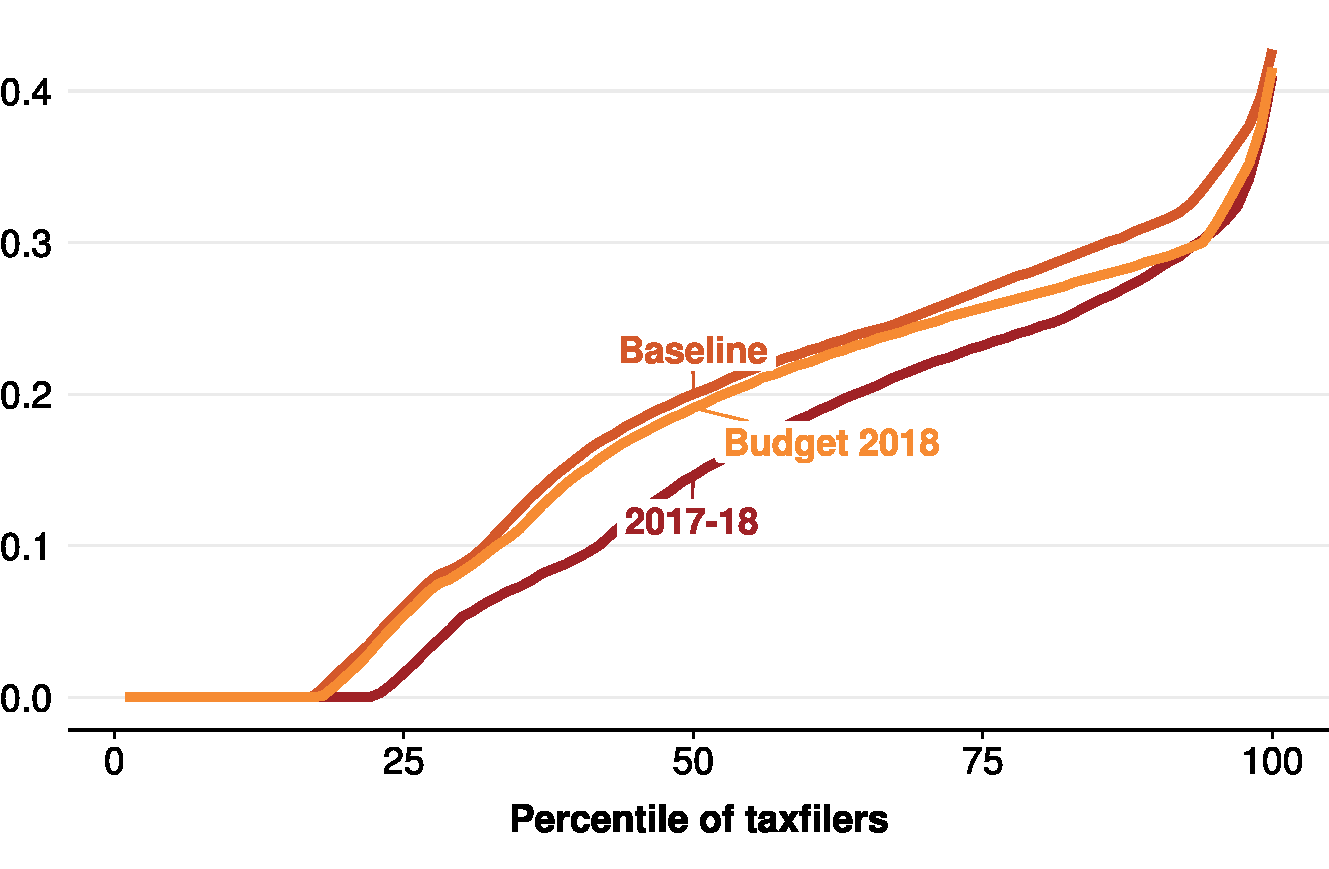
\includegraphics[width=4.47222in,height=2.92631723826715in]{atlas/fig2-1} 

\end{knitrout}

\source{\textcite{ATO2018}; Grattan analysis}
\end{figure}

Once fully implemented, the Tax Plan won't have much impact on the progressivity of the tax system. Overall, those on high incomes will pay a similar proportion of total tax revenues with or without the Tax Plan. But because of bracket creep in the meantime, high-income earners will be paying a lower proportion of income tax than today.

Under the Tax Plan, a person who earns \$120,000 today (more than 90 per cent of other income earners) will pay an average tax rate of 29 per cent in 2027-28, unchanged from today. In contrast, average tax rates for middle-income earners will be higher. The average tax rate for a taxpayer who earns \$36,000-a-year today (more than 40 per cent of other taxpayers) will increase 6 percentage points (from 10 to 16 per cent).

As a result, about 3 per cent of the tax burden will be shifted from the top 20 per cent of income earners to everyone else, as shown in \Vref{tbl:1}. Analysis of \emph{household} quintiles provides similar results, although this is less fine-grained than our analysis of taxpayers.\footcite{Phillips2018}

One published analysis of all adults appears to differ. It suggests that the top 20 per cent of adults -- approximately the top 40 per cent of taxfilers -- will pay a greater percentage of income tax in 2024-25 than in 2017-18,\footcite{Greber} but to date we have been unable to reproduce this analysis with publicly available data.

Overall, the Tax Plan itself has a similar effect on most taxfilers. The various components of the package collectively reduce average tax rates by around 2 percentage points for almost all taxpayers in a way that is so remarkably flat that it looks as though they were designed that way -- and perhaps they were. The only exception are the top 1 per cent get less of a tax cut as a proportion of their income, while the top 2 to 6 per cent get a bit more, as shown in \Vref{fig:3}.

\begin{figure}
\caption{Bracket creep hurts middle incomes most; the Tax Plan provides similar relief across the board apart from the top two deciles}\label{fig:3}
\units{Percentage point change in average tax rates, by taxable income percentile}
\begin{knitrout}
\definecolor{shadecolor}{rgb}{0.969, 0.969, 0.969}\color{fgcolor}
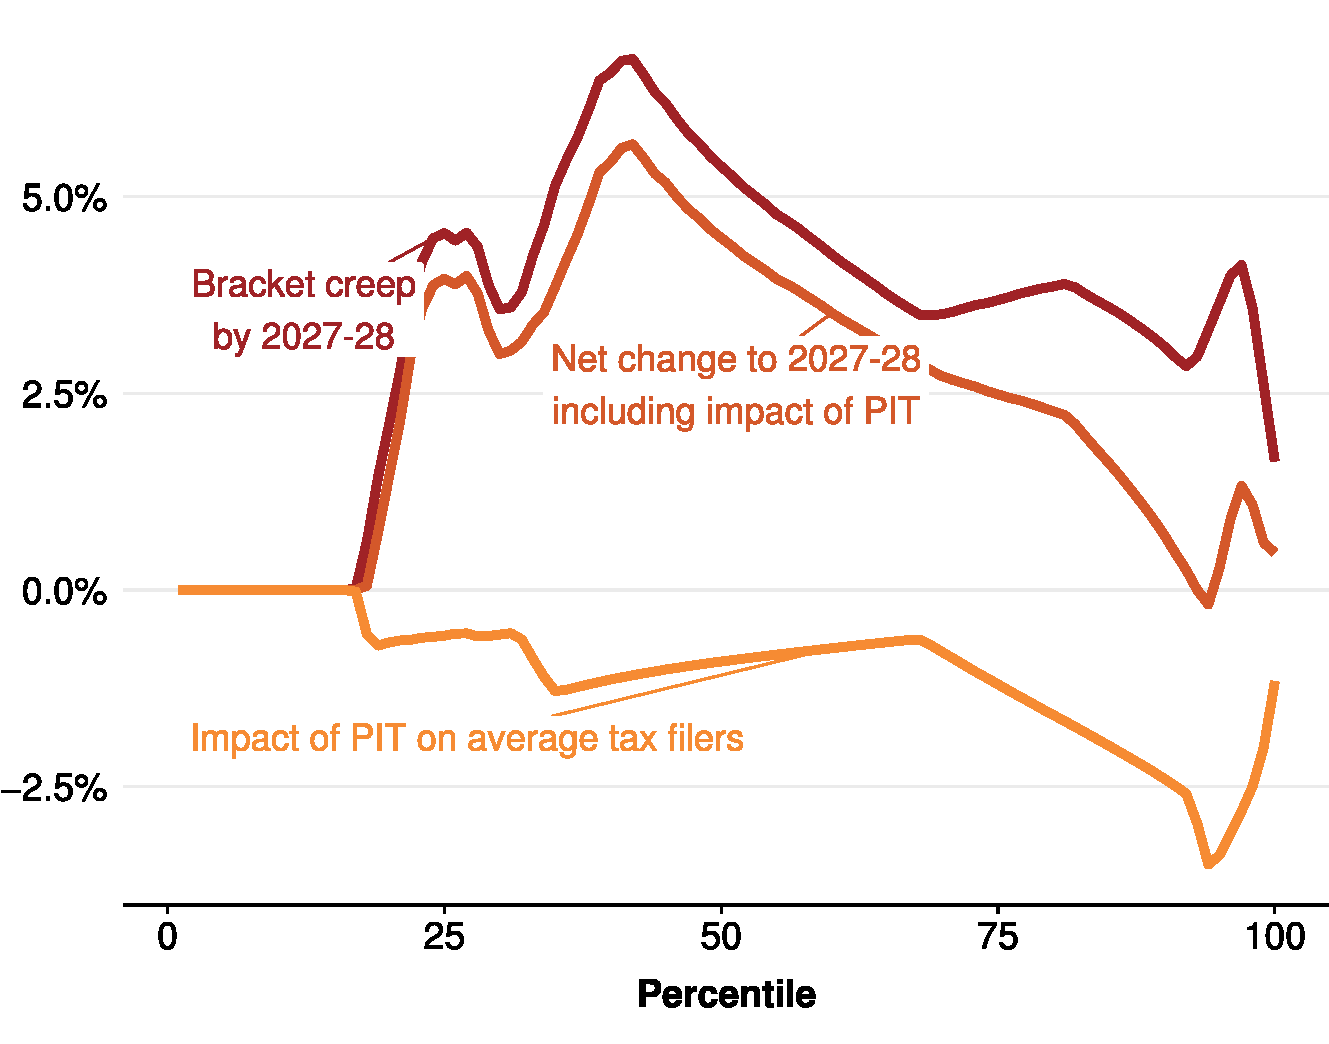
\includegraphics[width=4.47222in,height=3.51158068592058in]{atlas/fig3-1} 

\end{knitrout}
\source{\textcite{ATO2018}; Grattan analysis}
\end{figure}

The overall progressivity of a tax system can be measured using the Reynolds-Smolensky index.  This calculates how much a tax system redistributes incomes.
As shown in \Vref{fig:progressivity}, on this measure the Australian income tax system became more progressive between 2012 and 2016. Without change, bracket creep will make the system less progressive. The first stages of the Tax Plan will make it more progressive; the final tranche will make it less progressive.


\begin{figure}
\caption{Using the Reynolds-Smolensky measure, bracket creep will make income tax less progressive; and the Tax Plan will make it worse}\label{fig:progressivity}
\units{Reynolds-Smolensky index of tax system progressivity (higher = more progressive)}
\begin{knitrout}
\definecolor{shadecolor}{rgb}{0.969, 0.969, 0.969}\color{fgcolor}
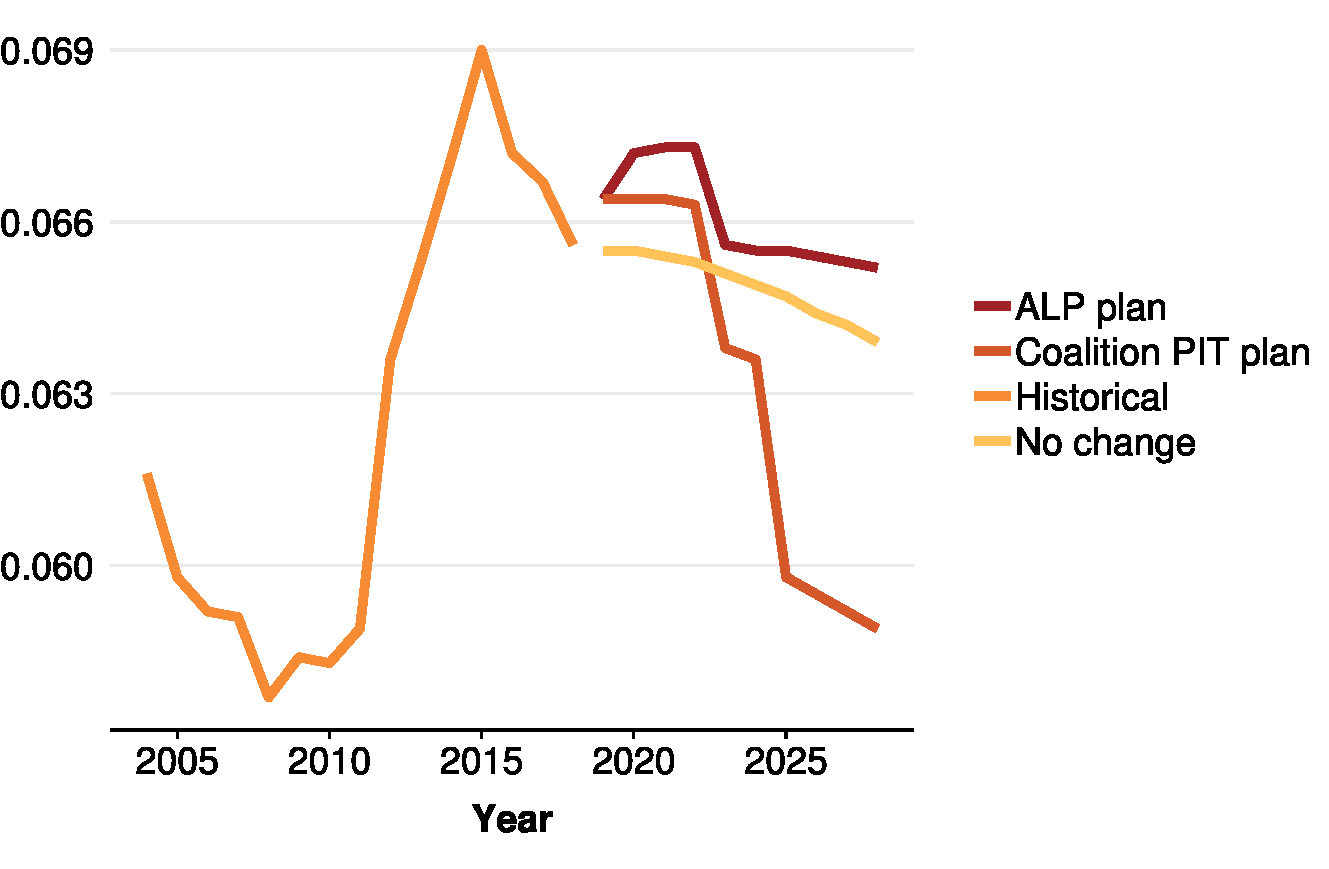
\includegraphics[width=4.47222in,height=2.92631723826715in]{atlas/progressivities-1} 

\end{knitrout}
\notes{Assumes ALP replicates Coalition tax plan for 2018-19. In 2019-20 ALP is assumed to offer a tax offset of \$350 a year to people earning less than \$37,000; between \$350 and \$928 a year for people earning between \$37,000 and \$48,000; the full \$928 a year for people earning between \$48,000 and \$90,000 and tapers at a rate of 2.625 cents per \$1 for people on incomes of between \$90,000 and \$125,333. Includes the increase in 37\% tax rate threshold from \$87,000 to \$90,000 from 2018-19.}
\source{\textcite{ATO2018}; Grattan analysis}
\end{figure}

\section{Sensitivity analysis}\label{sec:sensitivity-analysis}

The impact of bracket creep and the tax package vary depending on future growth in incomes. Our analysis has assumed the wages growth projected in the 2018-19 Budget, of 3.5 per cent per year from 2020-21.%
  \footcite[][1--10]{Treasury2018a}
Many have suggested that this is too high, given much lower wages growth in Australia and around the world for an extended period.\footnote{For example, \textcite{Knaus}.}

If income growth is lower, then bracket creep will be less regressive, as \Vref{fig:progressivity} shows. The effect of lower wage growth on the Tax Plan will be mixed: it will give more to low-income households (who stay within the expanded Low Income Tax Offset); and help those in the 7\textsuperscript{th} 8\textsuperscript{th} and 9\textsuperscript{th} deciles less (because they will get less benefit from the reduction in tax rate to 32.5c for incomes over \$87,000). Overall, bracket creep and the Tax Package will reduce the progressivity of the system a little less than if wage growth is at 2.75 per cent rather than 3.5 per cent as projected by the Budget.

\section{Other analysis}\label{sec:other-analysis}

Other analysis has highlighted that without the Tax Plan, ``average and middle-income earners'' -- \ie~those earning the equivalent of \$76,000 a year today -- will be in a higher tax bracket.
  \footcite{Benson}
But such analysis proves nothing about the fairness or otherwise of the tax package.

Those earning \$76,000 today earn more than 75~per~cent of income earners -- they are hardly ``middle income'' earners.

And even if such people have moved into a higher tax bracket, bracket creep will continue to have more effect on lower-income earners.

\vspace{3\baselineskip}


\begin{table}[H]
\caption{Lower wages growth would make bracket creep and the Tax Package less regressive over the decade}\label{tbl:2}
% latex table generated in R 3.5.0 by xtable 1.8-2 package
% Sun Jun 03 21:44:50 2018
\begin{tabularx}{\textwidth}{rRRRRRR}
  \toprule
   & \multicolumn{3}{c}{\textbf{Budget assumptions}} & \multicolumn{3}{c}{\textbf{2.75\% wage growth}}\\
 \cmidrule(lr){2-4}\cmidrule(lr){5-7}
 \textbf{Decile} & \textbf{2017-18} & \textbf{2027-28 baseline} & \textbf{2027-28 budget} & \textbf{2017-18} & \textbf{2027-28 baseline} & \textbf{2027-28 budget}\\
 \midrule
1 & 0\% & 0\% & 0\% & 0\% & 0\% & 0\% \\ 
  2 & 0\% & 0\% & 0\% & 0\% & 0\% & 0\% \\ 
  3 & 0.4\% & 0.8\% & 0.8\% & 0.4\% & 0.8\% & 0.7\% \\ 
  4 & 1.6\% & 2.3\% & 2.3\% & 1.6\% & 2.2\% & 2.1\% \\ 
  5 & 3.4\% & 4.3\% & 4.3\% & 3.4\% & 4.2\% & 4.2\% \\ 
  6 & 5.8\% & 6.3\% & 6.4\% & 5.8\% & 6.2\% & 6.3\% \\ 
  7 & 8.5\% & 8.7\% & 8.9\% & 8.5\% & 8.6\% & 8.9\% \\ 
  8 & 12.1\% & 12.2\% & 12.3\% & 12.1\% & 12.1\% & 12.3\% \\ 
  9 & 17.8\% & 17.9\% & 17.7\% & 17.8\% & 17.8\% & 17.7\% \\ 
  91-99 perc. & 32.9\% & 32.2\% & 31.5\% & 32.9\% & 32.3\% & 31.5\% \\ 
  1\% & 17.5\% & 15.3\% & 15.9\% & 17.5\% & 15.8\% & 16.3\% \\ 
   \bottomrule
\end{tabularx}

\end{table}
\printbibliography
\end{document}
